% !TEX root = ./main.tex
\documentclass[a4paper]{article}
% Course language: use [english] or [german].
\usepackage[german]{ajnotes}
\title{\textbf{Betriebwirtschaftslehre — Woche 2}}
\begin{document}
    \maketitle
    % Attach the given problem sheet: drop it in this folder as sheet.pdf and
    % un-comment the next line (pdfpages is already loaded by the preamble).
    % \includepdf[pages=-]{sheet.pdf}
    \textbf{Unterlagen} \url{https://lms.uzh.ch/auth/RepositoryEntry/17910989063/CourseNode/82241834376143}
    \section{Bestandteile des Gründungsmanagements}
    Schuhimport Unternehmen, Kunden in Zuri. Es mangelt am Startkapital
    \subexercise{a} Anpruchsgruppen (Stakeholder) und deren Ziele.
    \begin{itemize}
        \item \textbf{Kunden} (qualitativ Hochwertiges Produkt inkl Support und Lieferung für möglichst geringen Preis)
        \item \textbf{Arbeiter} (gute Arbeitsbedingungen, und Löhne)
        \item \textbf{Lieferanten} (Interessiert an erfolg der Lieferkette und Zuverlässige Verträge)
        \item \textbf{Investoren FK} (Hohe Renditen, Wiederaeusserbarkeit, Geringes Risiko oder Transparenz)
        \item \textbf{Gründerteam EK} (Erhöhung Markteintrittsbarrieren, basically gleich wie Fremdinvestoren)
    \end{itemize}

    \subsection{Beziehungen Zwischen Anpruchsgruppenziele}
    \begin{itemize}
        \item Komplementär
        \item konkurrierend
        \item indifferenz (keine Interferenz)
    \end{itemize}
    \subsection{Gruendungsprozess}
    \begin{enumerate}
        \item Konzeption
            \subitem Sammlung von Fremdkapital Ueberzeugung Investoren
        \item Planung
            \subitem Finanz. Entscheidungen 
        \item Wachstum
            \subitem Realisierung Umsetzung 
        \item Exit (Verkauf)
    \end{enumerate}

    \subsection{Methoden Ideensfindung und -evaluierung}
    \begin{enumerate}
        \item Erste neue lösung erfinden zu einem Gemeinschaftlichen Problem
        \item Eigenes Problem loesen
        \item Bestehendes qualitativ Verbessern
        \item Bestehendes quantitativ Billiger machen (produktivitätserhöhung oder qualitätserniedrigung)
    \end{enumerate}

     \textbf{Rekombination} ("nur 5\% sind originelle neue ideen")
    \begin{itemize}
        \item Konzeptübertragung (Disposable razorblades zu Disposable Kaffeekapseln)\footnote{Super fürs geschäft und für die umwelt}
        \item Kombinierung
        \item Wiederholung
    \end{itemize}

    \subsection{Evaluationskriterien}
    \textit{Siehe figures unternhemens\_evaluationsraster}
    \begin{enumerate}
        \item Kundennutzen
        \begin{itemize}
            \item Selbstverständlichkeit für Kunde welche Probleme/Beduerfnisse es löst/befriedigt
            \item Differenzierung qualitativ oder quantitativ
                \subitem \textbf{USP} Unique Selling Proposition  
        \end{itemize}
        \item Markt und Wettbewerb
        \subitem Markt
        \begin{itemize}
            \item Hinreichender Gesamtmarktgrösse
            \item Marktwachstumschangen vorhanden
        \end{itemize}
        \subitem Wettbewerb
        \begin{itemize}
            \item Differenzierung [nochmals..]
            \item Keine qualitativ Verschiedene Ersatzprodukten (Konkurrenten können gleiches und mehr)
            \item Hohe Immitations- Markteintrittsbarrieren \footnote{Alle verteidigen den "freien Markt" solange sie die Wettbewerbsstärksten sind.s}
            \item Kostenvorteile relativ zur Konkurrenz
        \end{itemize} \break
        \item Ertragsmechanik
        \begin{itemize}
            \item Möglichkeit zur Gewinnmaximierung
            \item Einnahmen aus konkreter Produkte und Dienste
            \item Einnahmen aus juristische Lizenzen und Werbespots 
            \begin{itemize}
                \item Free 1 Brindes und Aktion (Buy 1 get 1)
                \item Free 2 - (Kunde (C) konsumiert gratis von (P) mit Werbungen (A))
                \item Free 3 - free Kunden von premium Kunden "subventioniert" 
                \item 4 Gift economy (einfacher Warenaustausch ohne Geldvermittelung)
            \end{itemize}
        \end{itemize}
    \end{enumerate}
    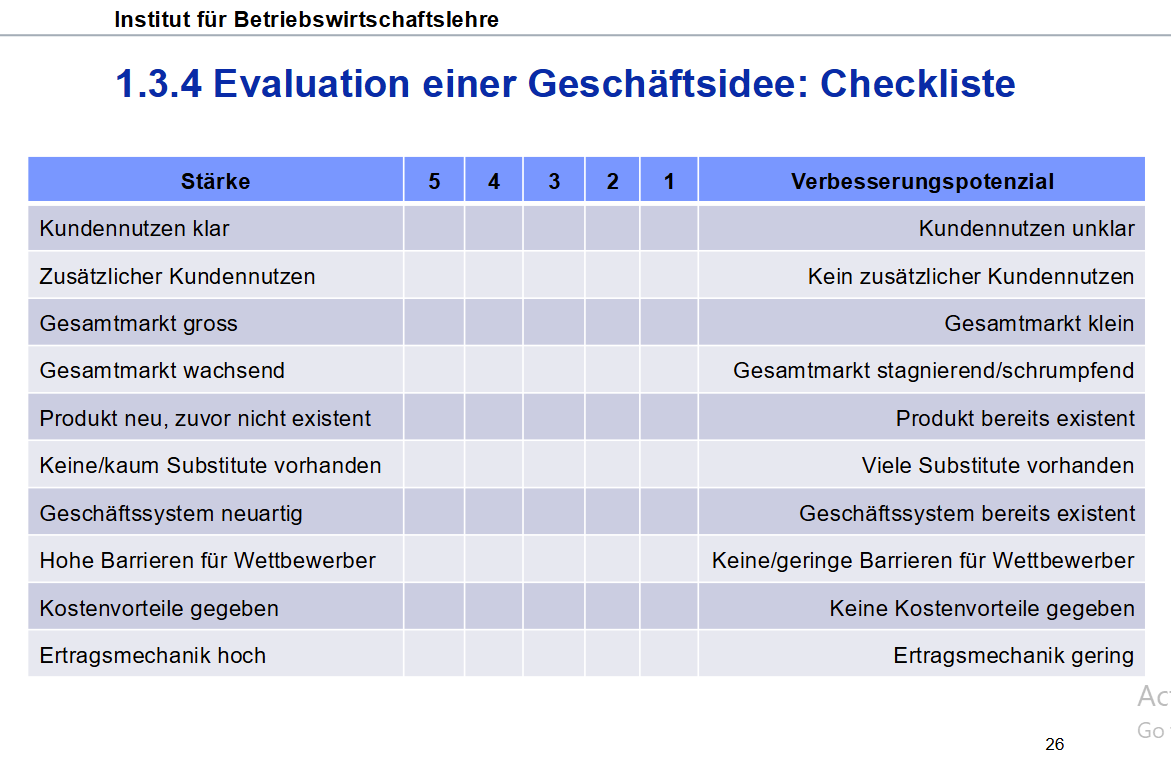
\includegraphics[width=\textwidth,height=0.7\textheight,keepaspectratio]{figures/unternehmens_evaluations_raster.png}
\end{document}
